
\documentclass{acmsiggraph}               % final
%\documentclass[review]{acmsiggraph}      % review
%\documentclass[widereview]{acmsiggraph}  % wide-spaced review
%\documentclass[preprint]{acmsiggraph}    % preprint

%% Uncomment one of the four lines above depending on where your paper is
%% in the conference process. ``review'' and ``widereview'' are for review
%% submission, ``preprint'' is for pre-publication, and ``final'' is for
%% the version to be printed.

%% These two line bring in essential packages: ``mathptmx'' for Type 1
%% typefaces, and ``graphicx'' for inclusion of EPS figures.

\usepackage{mathptmx}
\usepackage{graphicx}
\usepackage{epsfig}
\usepackage{amsmath,amscd,amssymb}

\newtheorem{theorem}{Theorem}[section]
\newtheorem{proposition}[theorem]{Proposition}
\newtheorem{definition}[theorem]{Definition}
\newtheorem{lemma}[theorem]{Lemma}
\newtheorem{corollary}[theorem]{Corollary}
\newtheorem{remark}[theorem]{Remark}


%% use this for zero \parindent and non-zero \parskip, intelligently.

\usepackage{parskip}

%% If you are submitting a paper to the annual conference, please replace
%% the value ``0'' below with your OnlineID. If you are not submitting this
%% paper to the annual conference, you may safely leave it at ``0'' -- it
%% will not be included in the output.

\onlineid{papers\_0142}

%% need to document this!

\acmformat{cameraready}

%% Paper title.

\title{Proposal: Visualizing the Loss Landscape of Neural Nets}

%% Author and Affiliation (single author).

%%\author{Roy G. Biv\thanks{e-mail: roy.g.biv@aol.com}\\Allied Widgets Research}

%% Author and Affiliation (multiple authors).

\author{Charles Ison\thanks{\small\texttt{e-mail: \{isonc|morgamat\}@eecs.oregonstate.edu}}\\ Oregon State University
\and Matthew Morgan$^{\ast}$ \\
Oregon State University}

%% Keywords that describe your work.

\keywords{rotational symmetry, field design, scalar field topology,
surfaces, topology.}

%%%%%% START OF THE PAPER %%%%%%

\begin{document}

\teaser{
%\centerline{\epsfig{file=images/teaser.eps,angle=0,width=\textwidth}}
    $\begin{array}{@{\hspace{-0.00in}}c@{\hspace{0.05in}}c@{\hspace{0.05in}}c@{\hspace{0.05in}}c}
    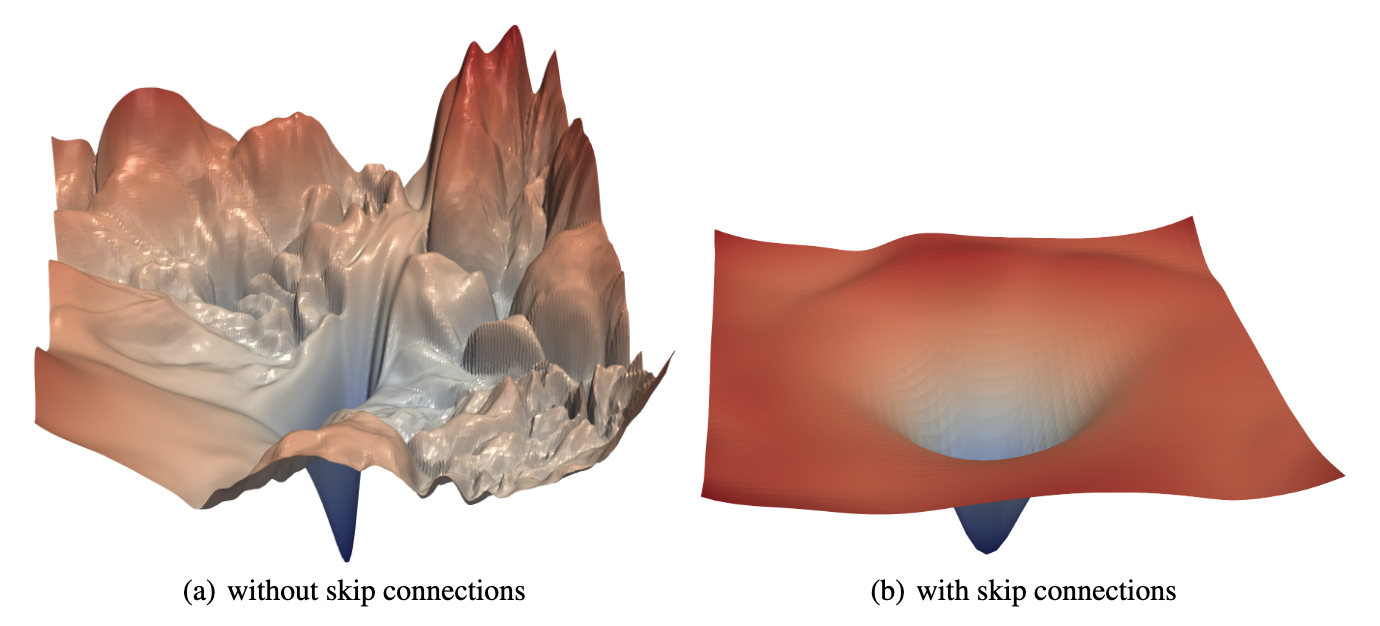
\includegraphics[width=5.50in]{/Users/mattm/repos/cs_453/sv_term_project/proposal/images/scalar-field-teaser.png}
    \\
    \end{array}$
\caption{Example of a loss landscape visualization from the paper: (a) without skip connections, (b)
with skip connections. } \label{fig:teaser} }

%% The ``\maketitle'' command must be the first command after the
%% ``\begin{document}'' command. It prepares and prints the title block.

\maketitle

%% Abstract section.

\begin{abstract}

\copyrightspace

Designing rotational symmetries on surfaces is a necessary task for
a wide variety of graphics applications, such as surface
parameterization and remeshing, painterly rendering and pen-and-ink
sketching, and texture synthesis. In these applications, the {\em
topology} of a rotational symmetry field such as {\em singularities}
and {\em separatrices} can have a direct impact on the quality of
the results. In this paper, we present a design system that provides
control over the topology of rotational symmetry fields on surfaces.

As the foundation of our system, we provide comprehensive analysis
for rotational symmetry fields on surfaces and present efficient
algorithms to identify singularities and separatrices. We also
describe design operations that allow a rotational symmetry field to
be created and modified in an intuitive fashion by using the idea of
basis fields and relaxation. In particular, we provide control over
the topology of a rotational symmetry field by allowing the user to
remove singularities from the field or to move them to more
desirable locations.

At the core of our analysis and design implementations is the
observation that $N$-way rotational symmetries can be described by
symmetric $N$-th order tensors, which allows an efficient
vector-based representation that not only supports coherent
definitions of arithmetic operations on rotational symmetries but
also enables many analysis and design operations for vector fields
to be adapted to rotational symmetry fields.

To demonstrate the effectiveness of our approach, we apply our
design system to pen-and-ink sketching and geometry remeshing.

\end{abstract}

%% ACM Computing Review (CR) categories.
%% See <http://www.acm.org/class/1998/> for details.
%% The ``\CRcat'' command takes four arguments.

\begin{CRcatlist}
  \CRcat{I.3.5}{Computer Graphics}{Computational Geometry and
Object Modeling}{Geometric algorithms, languages, and systems};
\end{CRcatlist}

%% The ``\keywordlist'' command prints out the keywords.
\keywordlist


\section{Introduction}
\label{sec:intro}


%% The ``\copyrightspace'' command must be the first command after the
%% start of the first section of the body of your paper. It ensures the
%% copyright space is left at the bottom of the first column on the first
%% page of your paper.


Many objects in computer graphics can be described by {\em
rotational symmetries}, such as brush strokes and hatches in
non-photorealistic rendering, regular patterns in texture synthesis,
and principle curvature directions in surface parameterization and
geometry remeshing. Intuitively, an {\em $N$-way rotational
symmetry} ($N$-RoSy) represents phenomena that are {\em invariant}
under rotations of an integer multiple of $\frac{2\pi}{N}$. Example
$N$-RoSy's include a vector ($N=1$), an eigenvector of a symmetric
matrix ($N=2$), and a cross ($N=4$). %Note we anticipate reflectional
%symmetries to be studied in the future, so we choose {\em RoSy} to
%distinguish.

\begin{figure*}[t]
\begin{center}
    $\begin{array}{@{\hspace{-0.00in}}c@{\hspace{0.05in}}c@{\hspace{0.05in}}c@{\hspace{0.05in}}c@{\hspace{0.05in}}c}
    
\includegraphics[height=1.3in]{images/tetra.eps}
    &
\includegraphics[height=1.3in]{images/octa.eps}
    &
\includegraphics[height=1.3in]{images/cube.eps}
    &
\includegraphics[height=1.3in]{images/icos.eps}
    &
\includegraphics[height=1.3in]{images/dodec.eps}\\
    \end{array}$
\end{center}
\caption{$N$-way rotational symmetries appear naturally in the
Platonic solids: tetrahedron ($N=2$), octahedron ($N=3$), cube
($N=4$), icosahedron ($N=6$), and dodecahedron ($N=10$). }
\label{fig:symmetry_examples}
\end{figure*}

Symmetries naturally appear in surfaces, such as the five Platonic
shapes (Figure~\ref{fig:symmetry_examples}). Notice that the order
of the symmetry $N$ is equal to the ratio between $2\pi$ and the
angle of deficit at a vertex. In surfaces where global symmetry is
lacking, local symmetries can still occur, such as the singularities
(the vertices). In Figure~\ref{fig:teaser} (c), singularities of a
$4$-RoSy field appear in natural places such as the corner of the
shoulder (not visible due to the highlight) and under the armpit.

The ability to design and control $N$-RoSy fields on surfaces is
essential in many applications. For example, in non-photorealistic
rendering, the orientation of brush strokes and hatches are usually
guided by an $N$-RoSy field. Different artistic effects can be
achieved by using guiding fields with different characteristics. In
addition, singularities in the guiding field can lead to visual
artifacts such as brush strokes and hatches with unnatural
orientations. Singularities also present difficulties in the
construction of a global surface parameterization, where a
significant amount of stretch can occur in nearby regions.
Similarly, it is difficult to produce ideal triangular and quad
elements near singularities in geometry remeshing. For these
applications, a design system can be used to create a wide variety
of $N$-RoSy fields on surfaces, to add desirable features in an
existing field, and to control the number and location of the
singularities in the field. Most existing design systems focus on
vectors
($N=1$)~\cite{Praun:00,Turk:01,Wei:01,Theisel:02,Stam:03,Zhang:06}
and tensors ($N=2$)~\cite{Zhang:07}. A number of difficulties must
be addressed before a general design system can be developed for $N
\ge 3$.

First, there has been a lack of a mathematical representation for
rotational symmetries, which is required to define algebraic
operations on $N$-RoSy's such as sums and scalar multiples as well
as important concepts of $N$-RoSy fields such as singularities,
continuity, and differentiability.
%One way to define the sum of two $N$-RoSy's $s_1$
%and $s_2$ is to find a vector in $s_1$, which is used to locate a
%vector in $s_2$ that has the minimum angular difference. The sum of
%two vectors is then defined to be a vector in $s_1 + s_2$. As
%illustrated in Figure~\ref{fig:question} (left and middle), this
%approach can lead to inconsistencies when interpolating among three
%$N$-RoSy, which is a common task.
We overcome this difficulty by embedding $N$-way rotational
symmetries in the space of $N$-th order tensors, which allows
algebraic operations to be carried over from $N$-th order tensors to
$N$-RoSy's. We further derive a vector-based representation of
rotational symmetries based on the embedding, which enables
efficient analysis of $N$-RoSy fields on surfaces as well as allows
vector field design functionalities to be adapted to $N$-RoSy
fields. Furthermore, the concepts of singularities, continuity, and
differentiability are well-defined.

Second, there is relatively little understanding of the topological
structure in an $N$-RoSy field. While the concepts of singularities
have been used before, a proper definition of separatrices is
missing when $N \ge 3$. To address this, we present efficient
algorithms on extracting the singularities and separatrices in a
field. In particular, we adopt the approach of Zhang et
al.~\shortcite{Zhang:06} that allows continuous $N$-RoSy fields to
be generated on mesh surfaces despite the discontinuity in the
surface normal.


With the above issues addressed, we present a design system for
$N$-RoSy fields on surfaces that not only allows a wide variety of
$N$-RoSy fields to be generated but also provides explicit control
over the number and location of the singularities in the field. The
main functionalities of our work is reminiscent of that for vector
field design~\cite{Zhang:06}. However, the implementations are
rather different. For instance, we can create an initial $N$-RoSy
field on a surface using relaxation techniques~\cite{Turk:01} which
do not require a global surface parameterization. This greatly
increases the interactivity of our system. We also reuse algorithms
for singularity pair cancellation and movement in vector fields
through the aforementioned vector-based representation.

We have applied our design system to graphics applications such as
pen-and-ink sketching and quad-dominant remeshing.

In this paper, we make the following contributions.

\begin{enumerate}
%\itemsep 0pt
%\parskip -1pt
\item We provide coherent definitions for algebraic
operations on $N$-RoSy's by observing the link between $N$-RoSy's
and $N$-th order symmetric tensors. This link also enables the
definitions of analytic properties of $N$-RoSy fields such as
continuity, differentiability, and singularity.
\item We present a vector-based representation for $N$-RoSy's that
supports compact storage of discrete $N$-RoSy fields on mesh
surfaces and facilitates the analysis and design of $N$-RoSy fields.
\item We describe the topology of $N$-RoSy fields on surfaces
and provide efficient algorithms to extract singularities and
separatrices.
\item We develop a design system in which $N$-RoSy fields
can be interactively created and modified on surfaces. In
particular, our system provides explicit control over the number and
location of the singularities in the field. We demonstrate the
effectiveness of our system with pen-and-ink sketching of surfaces
and quad-dominant remeshing.
%\item We present a visualization technique that is fast and
%high-quality when $N=2$, $3$, $4$, and $6$.
\end{enumerate}

The remainder of the paper is organized as follows. We first review
related work on $N$-RoSy fields in Section~\ref{sec:previous_work}
and present our vector-based representation of $N$-RoSy's in
Section~\ref{sec:representation}. Next, we discuss the analysis and
design of $N$-RoSy fields in Sections~\ref{sec:analysis}
and~\ref{sec:design}, respectively. In
Section~\ref{sec:application}, we show the results of applying our
analysis and design system to pen-and-ink sketching and geometry
remeshing. Finally, we summarize our contributions and discuss some
possible future work in Section~\ref{sec:conclusion}.

\section{Previous Work}
\label{sec:previous_work}

There has been a significant amount of work in the analysis and
design of vector and tensor fields. In contrast, relatively little
is known about $N$-RoSy fields when $N \ge 3$.

{\bf $N$-RoSy Analysis and Design:} To the best of our knowledge,
Hertzmann and Zorin~\shortcite{Hertzmann:00} are the first to
propose that hatches should follow a cross field ($4$-RoSy). They
provide a smoothing operation on $4$-RoSy fields that is based on a
non-linear optimization. Ray et al.~\shortcite{Ray:06} construct a
periodic global parameterization that facilitates quad remeshing. At
the heart of their approach is the use of $4$-RoSy fields, which
allows more natural-shaped quads to be generated near singularities.
They also develop a framework that allows the optimization to be
performed on the sines and cosines of the parameterization, which
turns a non-linear optimization into a linear one. They later
provide the analysis of singularities on $N$-RoSy's by extending the
Poincar\'e-Hopf theorem as well as describe an algorithm in which a
field with a minimal number of singularities can be constructed
based on user-specified constraints and the Euler characteristic of
the underlying surface~\cite{ray:07}.

{\bf Vector and Tensor Field Design:} There have been a number of
vector field design systems for surfaces. Most of them are generated
for a particular graphics application such as texture
synthesis~\cite{Praun:00,Turk:01,Wei:01}, fluid
simulation~\cite{Stam:03}, and vector field
visualization~\cite{vanWijk:02,vanWijk:03}. These systems do not
address topological control in the field. Systems providing
topological control include~\cite{Theisel:02,Zhang:06}. The system
of Zhang et al. has also been extended to create periodic
orbits~\cite{Chen:07} and to design tensor fields~\cite{NEURIPS2018_a41b3bb3}.
Our system is also reminiscent of the vector field design system of
Zhang et al.~\shortcite{Zhang:06} in terms of the functionality.
However, the implementation is rather different.

{\bf Vector and Tensor Field Analysis:} There has been much work in
vector and tensor field analysis. To review all the work is beyond
the scope of this paper. Here we refer to the most relevant work.
Helman and Hesselink~\shortcite{Helman:91} propose vector field
visualization techniques based on topological analysis. Delmarcelle
and Hesselink provide analysis of second-order symmetric tensor
fields~\shortcite{NEURIPS2018_a41b3bb3}.

%Cabral and Leedom present a texture-based visualization for vector
%fields, which they termed {\em LIC} (Line-integral
%convolution)~\cite{Cabral:93}. This technique is of high quality.
%Later, van Wijk~\shortcite{vanWijk:02,vanWijk:03} provides an
%image-based flow visualization technique (IBFV) that is of similar
%quality but much faster due to the use of graphics hardware. Zhang
%et al.~\shortcite{Zhang:07} extend IBFV to symmetric second-order
%tensor fields.

\section{Vector-Based Representation}
\label{sec:representation}

TODO...



\begin{figure}[t]
\begin{center}
    $\begin{array}{@{\hspace{-0.00in}}c@{\hspace{0.05in}}c}
    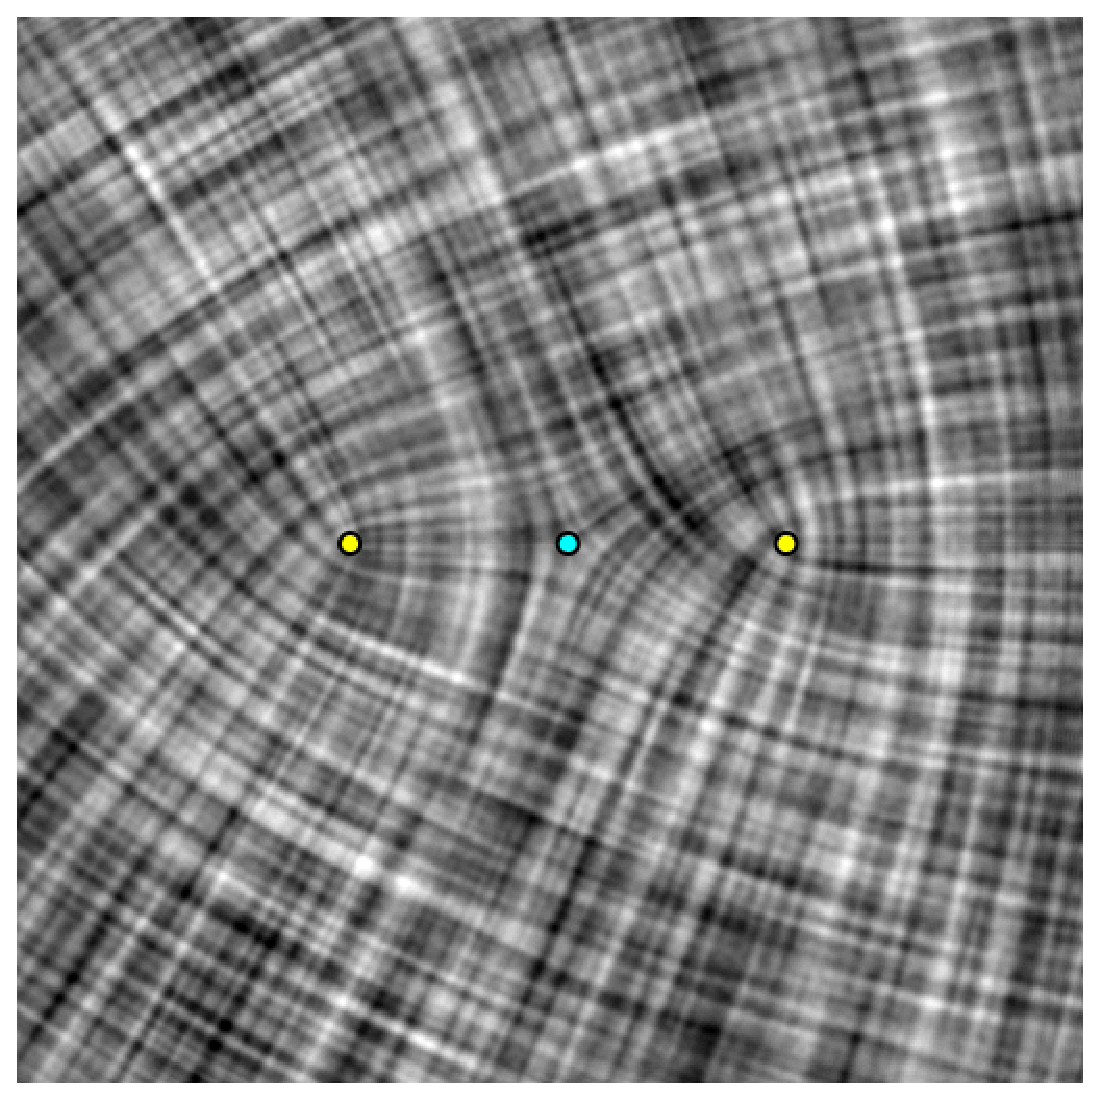
\includegraphics[height=1.07in]{images/cancel_step0_4sym.eps}
    &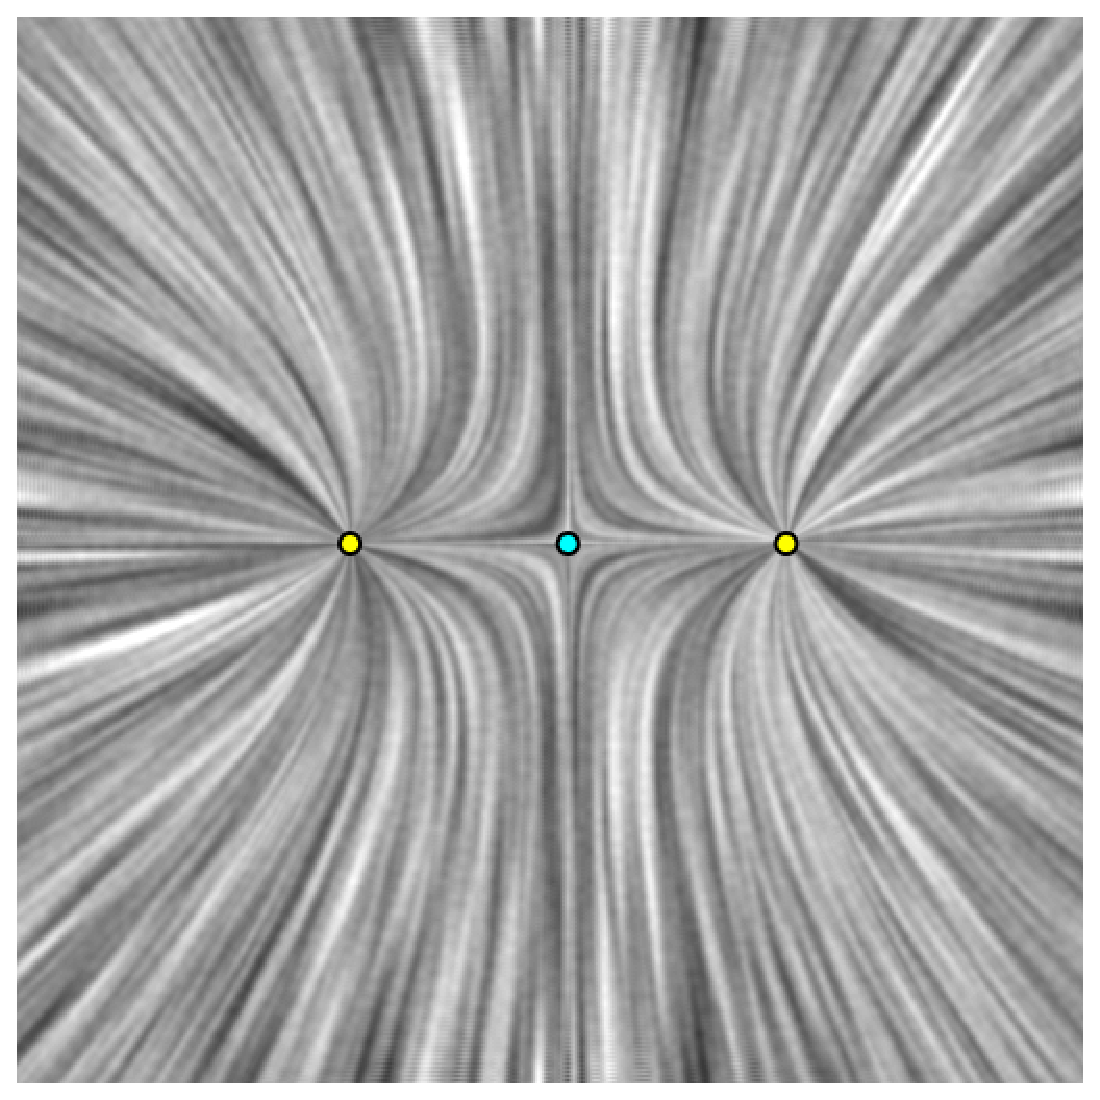
\includegraphics[height=1.07in]{images/cancel_step0_1sym.eps}
    \\
    \end{array}$
\end{center}
\caption{ A comparison between a $4$-RoSy field (left) and its
representation vector field (right). Notice that the sets of points
with a zero value are the same for both fields (colored dots).
Representation vectors remove the directional ambiguity in an
$N$-RoSy field. } \label{fig:vector_representation}
\end{figure}

\section{Topological Analysis of $N$-RoSy Fields}
\label{sec:analysis}

In this section, TODO...

\section{Design of $N$-RoSy Fields}
\label{sec:design}

In this section, TODO\dots



\section{Applications}
\label{sec:application}

We have applied our design system to pen-and-ink sketching and
quad-dominant remeshing.


\subsection{Example Subsection}
\label{sec:pen_and_ink}

Subsection, TODO\dots



\section*{Appendix: $N$-RoSy's and $N$-th Order Tensors}
\label{sec:higher_tensors}

To be determined.

\section*{Acknowledgements}

To be determined.


\bibliographystyle{acmsiggraph}
\nocite{*}
\bibliography{nn_loss}
\end{document}
